The design of high-frequency magnetic components is strictly dictated by the electrical specifications of the target power conversion system. This research is driven by demands for high-power, high-frequency SSTs and other applications that require the said architecture, which includes fast-charging infrastructure and energy distribution systems. This chapter details insights regarding the selection of the application topology for the proposed isolation transformer.

\section{System Specifications}
Based on the established research demands, the target electrical parameters for the isolation stage DC--DC converter are as shown in Table \ref{tab:converter_specs}. Operating within these regimes requires a converter topology that can minimize switching losses while accommodating the isolation stage transformer.

\begin{table}[h!]
\centering
\caption{Established Converter Specifications}
\label{tab:converter_specs}
\begin{tabular}{cccc}
\hline
\textbf{Parameter} & \textbf{Symbol} & \textbf{Value} \\
\hline \hline
Input Voltage & $V_{\mathrm{in}}$ & nom. 1000 V \\ 
Output Voltage & $V_{\mathrm{out}}$ & 1000 V   \\
Switching Frequency & $f_{\mathrm{sw}}$ & 15 -- 30 kHz \\ 
Output Power & $P_\mathrm{O}$ & 100 kW \\
Output Current & $I_\mathrm{O}$ & 100 A \\
\hline
\end{tabular}
\end{table}

In this study, due to the capabilities of the researchers and laboratory, and especially that the research first requires a proof of concept, a scaled down version of the system is first examined, equally scaling down current and voltage by 10 each to reach a baseline nominal operating condition of 100 V: 100 V, 1 kW, under the same operating frequency condition. The transformer turn ratio $n$ is set to 1.

\section{Considered High Power Topologies}
In SST applications, most topologies should have bidirectional capability to allow interoperation between the grid and its consumers. Selecting the optimal isolated bidirectional DC--DC converter topology is a critical first step, and most topologies in this application use the Dual Active Bridge (DAB) Converter and the Capacitor-Inductor-Inductor-Capacitor (CLLC) resonant converter. Their circuit diagrams are shown in Figure \ref{fig:DAB} and Figure \ref{fig:CLLC}. 

\begin{figure}[h!]
    \centering
    \subfloat[]{
        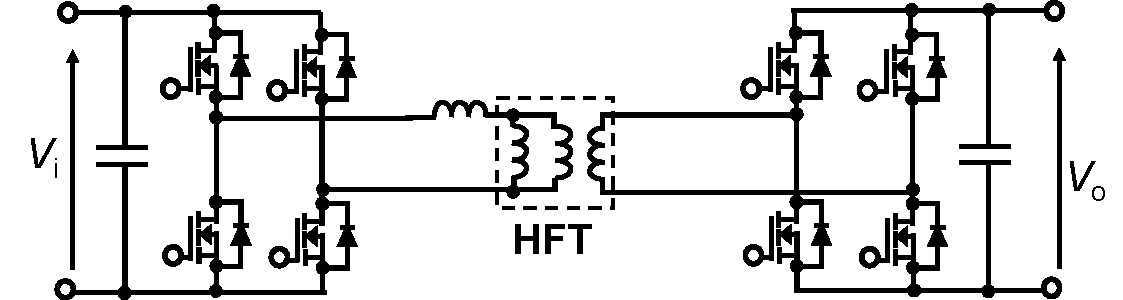
\includegraphics[width=0.8\columnwidth]{figures_chapter2/DAB.pdf} \label{fig:DAB}
    }
\\
     \subfloat[]{
        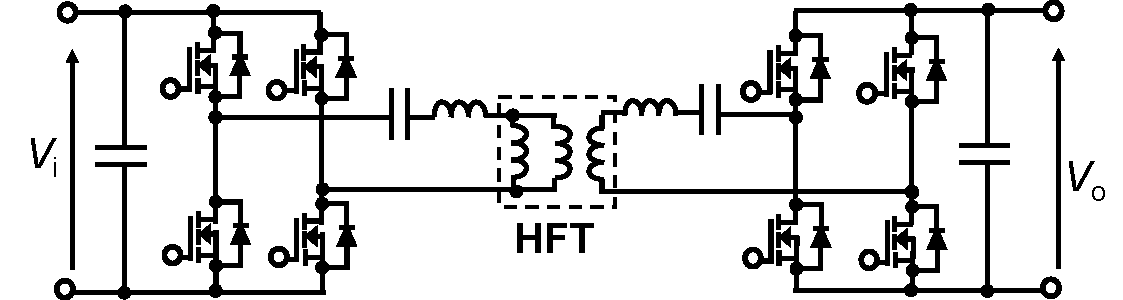
\includegraphics[width=0.8\columnwidth]{figures_chapter2/CLLC.pdf} \label{fig:CLLC}
    }
\caption{Bidirectional converters for SST applications: (a) the Dual Active Bridge (DAB) converter, and (b) the Capacitor-Inductor-Inductor-Capacitor (CLLC) resonant converter.}
\end{figure}


\begin{figure}[H]
    \centering
    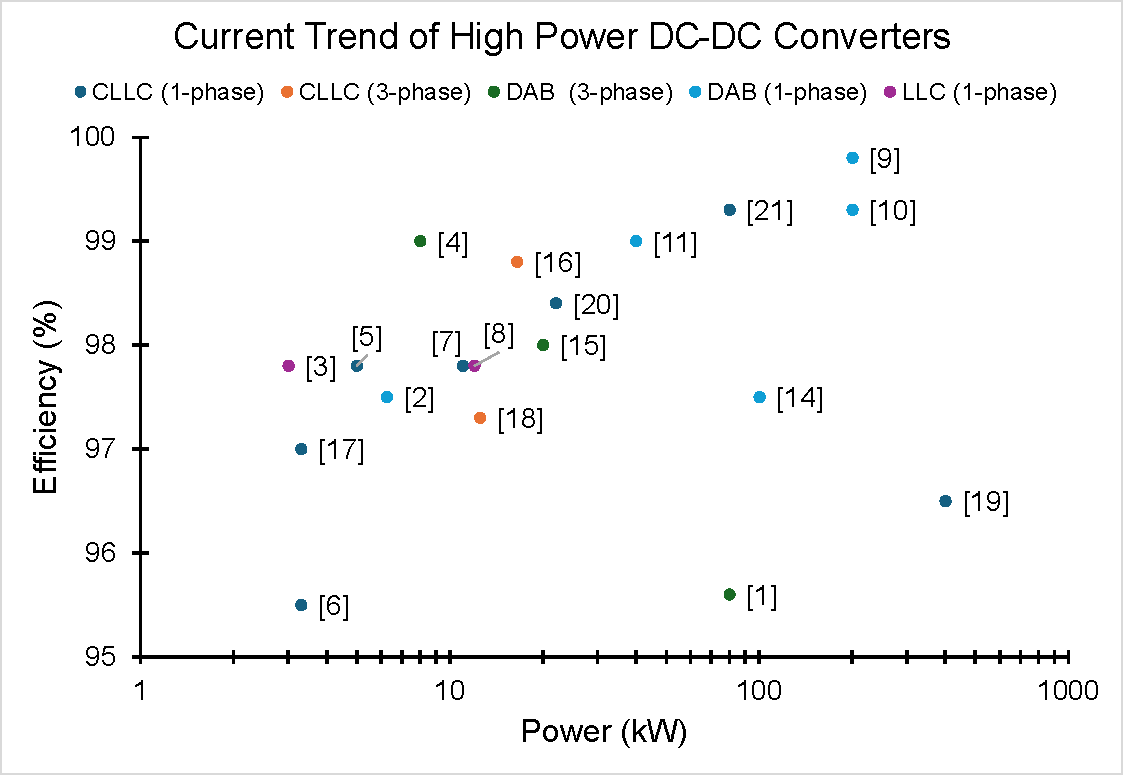
\includegraphics[width=0.8\columnwidth]{figures_chapter2/HighPower.pdf}
    \caption{A compilation of high power converters at different power levels. The data utilized can be seen in the Appendix: \nameref{app:converter_trends}.}\label{fig:HighPower}
\end{figure} 
A compilation of the current trend of high-power converters is shown in Figure \ref{fig:HighPower}. Most high power converters in SST Applications utilize the DAB. This is due to their versatility and ease of operation and control. However, the DAB is prone to DC Bias due to the control scheme used \cite{zhang2019analog}. Eliminating DC Bias is important as it can resolve to core saturation, which can then cause excessive heating, loss, and disruption to circuit operation. Moreover, it is also known to have a narrow ZVS range and higher peak current when the phase shift increases, leading to more losses \cite{krismer2012efficiency}. 

To overcome these limitations, the bidirectional CLLC resonant converter is selected for this study. The CLLC topology integrates a symmetric resonant tank on both the primary and secondary sides of the high-frequency transformer. It is also known to have a wider range of ZVS operation even at lighter loads, which can improve efficiency in the overall operating range. It utilizes resonance and the magnetizing inductance to store and transfer energy through the fine tuning of operation frequency. However, it is difficult to implement frequency control, and careful tuning of the two resonant tanks. Moreover, higher peak operational current is expected, which can cause more component stress \cite{ref19, mukherjee2021comparison}. 

A short summary comparing each topology is shown in Table \ref{tab:tabcomparison}. 

\begin{table}[h!]
\centering
\caption{Comparison of DAB and CLLC Resonant Converters \cite{mukherjee2021comparison, oh2024comparison}} \label{tab:tabcomparison}
\label{tab:dab_vs_cllc}
\begin{tabular}{
    >{\raggedright\arraybackslash}p{0.22\textwidth} 
    >{\raggedright\arraybackslash}p{0.35\textwidth} 
    >{\raggedright\arraybackslash}p{0.35\textwidth}
}
\hline
\textbf{Parameter} & \textbf{Dual Active Bridge Converter \cite{krismer2012efficiency, costa2015modular, anwar2018modeling}} & \textbf{CLLC Resonant Converter \cite{ref19, xie2019analysis}} \\
\hline \hline

\textbf{Efficiency} & 
Peak efficiency is achieved near nominal load; efficiency degrades significantly under light loads due to circulating currents. & 
Maintains high efficiency across a substantially wider load range due to minimized switching and circulating losses. \\

\textbf{Control Strategy} & 
Phase-Shift Modulation (PSM); conceptually straightforward but requires highly precise timing synchronization between bridges. & 
Pulse Frequency Modulation (PFM); regulates voltage gain effectively without relying on complex cross-isolation communication. \\

\textbf{Soft-Switching (ZVS)} & 
ZVS region is constrained; often lost under light-load conditions or non-unity voltage gains. & 
Inherent ZVS capability is maintained seamlessly across a wide operating region for both forward and reverse power flow. \\

\textbf{Current Characteristics} & 
Trapezoidal current profile; minimizes RMS currents only when operating under optimal, low phase-shift conditions. & 
Sinusoidal current profile; inherently results in higher RMS currents compared to an optimized DAB. \\

\textbf{Component Stress} & 
High circulating reactive currents and elevated core losses when operating away from the optimal design point. & 
Higher peak operational currents impose stricter thermal and electrical stress ratings on semiconductor devices. \\

\textbf{Component Count \& Complexity} & 
8 switches and 1 series transfer inductor (typically integrated utilizing the transformer's leakage inductance). & 
8 switches, plus primary and secondary resonant capacitors. Sourcing AC capacitors for high-voltage/high-current ratings can increase volume and cost. \\

\textbf{Target Applications} & 
Ideal for fixed-voltage-ratio (DCX) applications prioritizing maximum full-load density and efficiency. & 
Ideal for bidirectional applications requiring wide input/output voltage regulation (e.g., EV chargers, SSTs). \\

\hline
\end{tabular}
\end{table}
\pagebreak
\section{The Bidirectional Resonant Converter}
\subsection{CLLC Operational Mode Analysis}
The bidirectional CLLC resonant converter operates through distinct topological states during each switching half-cycle \cite{infineon_cllc, ref19}. In this explanation, operation is assumed at or near the resonant frequency. Moreover, for brevity, the operational analysis is performed only for the first pair of switches, $S_1$ and $S_4$, operating in forward power delivery. This then means that the secondary side switches are off and are in rectification operation. The process is symmetrical for the other pair of switches, and also for reverse power delivery. An illustration of the first three modes of operation is shown in Figure \ref{fig:operation} and the key waveforms are shown in Figure \ref{fig:keywaveform}.
\begin{figure}[h!]
    \centering
    \subfloat[]{
        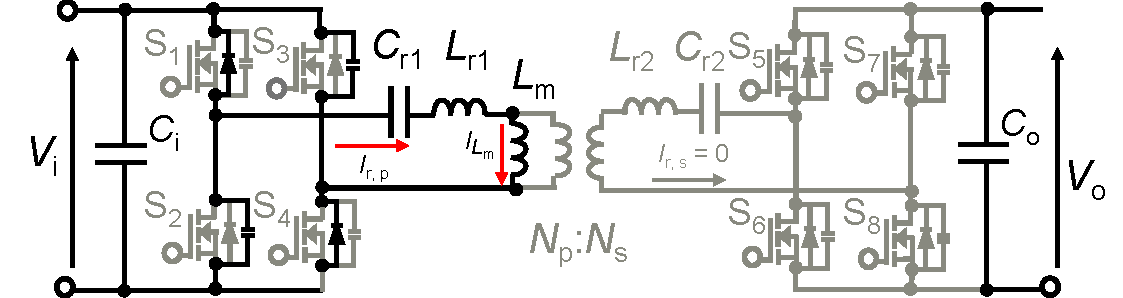
\includegraphics[width=0.8\columnwidth]{figures_chapter2/mode1.pdf} \label{fig:mode1}
    }
\\
     \subfloat[]{
        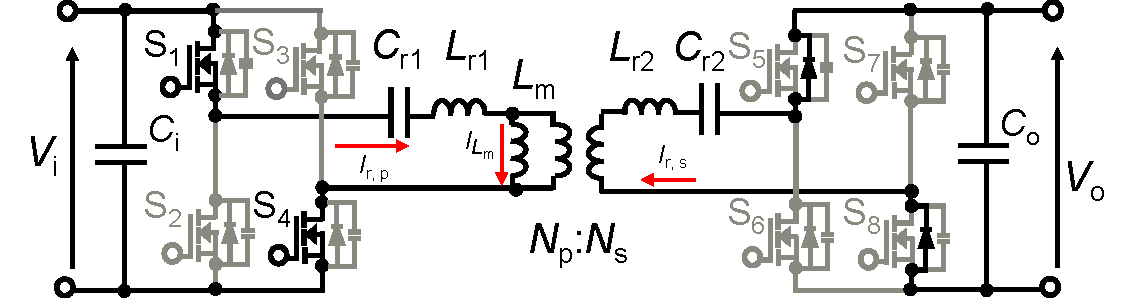
\includegraphics[width=0.8\columnwidth]{figures_chapter2/mode2.pdf} \label{fig:mode2}
    }
\\
     \subfloat[]{
        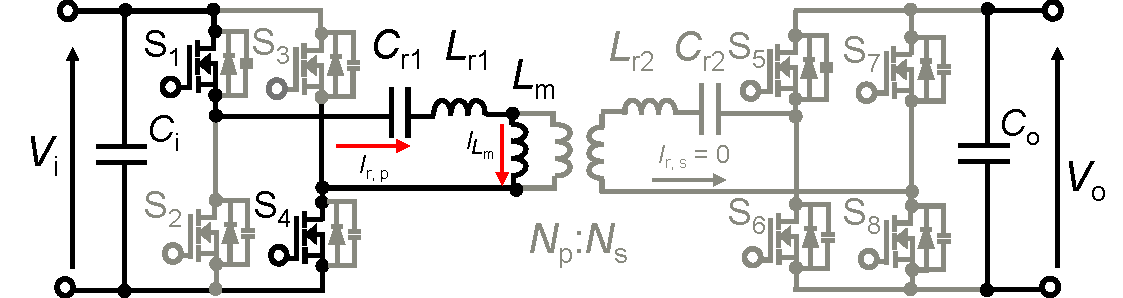
\includegraphics[width=0.8\columnwidth]{figures_chapter2/mode3.pdf} \label{fig:mode3}
    }
\caption{First three modes of operation of the CLLC: (a) State 1 $t_1<t<t_2$, (b) State 2 $t_2<t<t_3$, and (c) State 3 $t_3<t<t_4$.} \label{fig:operation}

\end{figure}

\begin{figure}[h!]
    \centering
    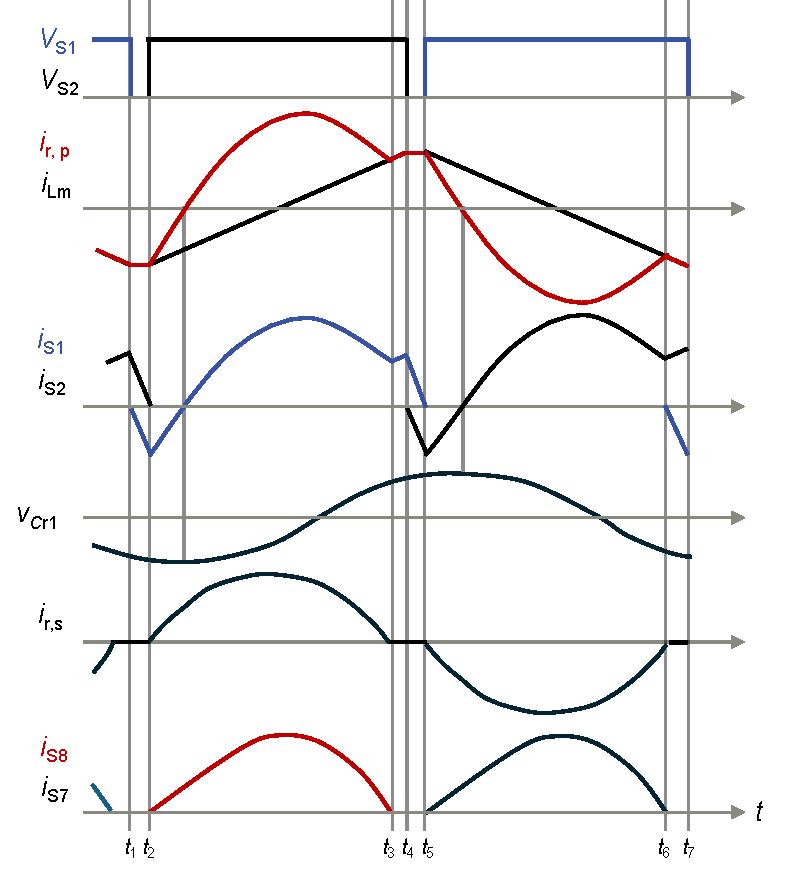
\includegraphics[width=0.8\columnwidth]{figures_chapter2/operational waveform.pdf}
\caption{Key waveforms of the CLLC.}\label{fig:keywaveform}
\end{figure}

\textbf{State 1 (Dead Time), $t_1<t<t_2$} (Figure \ref{fig:mode1}) :
All switches are off to avoid overshoot. During the dead-time duration, no power is transferred to the secondary side. The primary resonance current $i_\mathrm{r, p}$ charges the output capacitances of switches $S_2$ and $S_3$ and discharges those of $S_1$ and $S_4$. After this process, $i_\mathrm{r,p}$ will pass through the diode of $S_1$ and $S_4$, which signifies ZVS.

\textbf{State 2 (Power Transfer Stage),  $t_2<t<t_3$} (Figure \ref{fig:mode2}):
Switches $S_1$ and $S_4$ turn on, enabling power transfer through the transformer. The primary side resonance current $i_\mathrm{r,p}$ changes direction, and the magnetizing inductance stores energy, as $i_{\mathrm{Lm}}$ rises linearly. This stage ends when $i_\mathrm{p}$ meets $i_\mathrm{Lm}$, signifying the end of the resonance operation.

\textbf{State 3 (Freewheeling State), $t_3<t<t_4$} (Figure \ref{fig:mode3}):
Because resonance operation is stopped, $i_\mathrm{r, s}$ is zero. This therefore means that $i_\mathrm{r, p}$ is also the same as $i_\mathrm{Lm}$, storing energy into the magnetizing inductance until $S_1$ and $S_4$ are turned off. When $L_\mathrm{m}$ is large enough, $i_\mathrm{r, p}$ follows $i_{\mathrm{Lm}}$ perfectly.

\subsection{CLLC First Harmonic Approximation (FHA)} \label{ref:FHA}
The First Harmonic Approximation (FHA) is a widely adopted analytical method for deriving the voltage gain and tuning the resonant tank parameters of the CLLC converter \cite{ref19}, \cite{infineon_cllc}. Because the resonant tank acts as a highly effective bandpass filter, the FHA method assumes that power transfer is overwhelmingly dominated by the fundamental harmonic component of the square-wave voltage generated by the active bridge. This then allows the circuit to be converted to an equivalent circuit with a sinusoidal input voltage and output as well. The equivalent input voltage $V_\mathrm{in, app}$, $V_\mathrm{o, app}$, and equivalent AC current $I_{\mathrm{ac}}$ are mapped out in both the original and equivalent circuit as shown in Figure \ref{fig:AC_orig} and Figure \ref{fig:AC_eq} respectively. The  AC resistance $R_{\mathrm{ac}}$ is the equivalent of the DC load with current $I_{\mathrm{o}}$ passing through it.

\begin{figure}[h!]
    \centering
    \subfloat[]{
        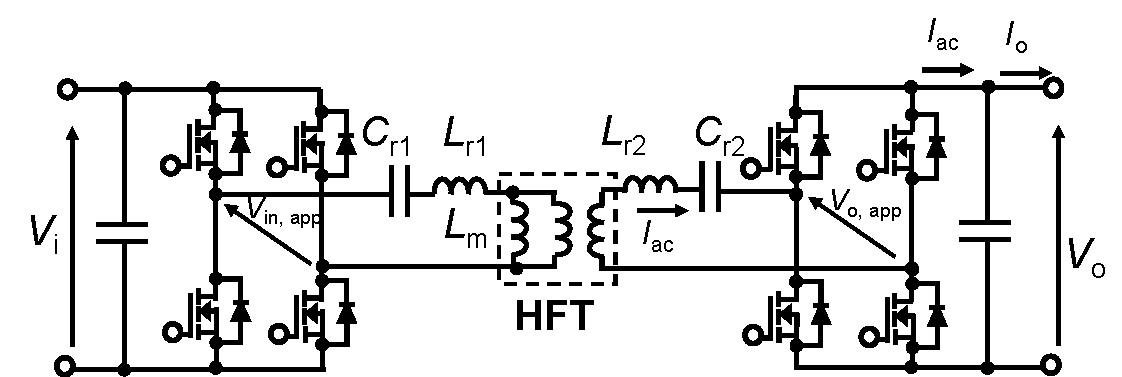
\includegraphics[width=0.9\columnwidth]{figures_chapter2/CLLC_FHA_full.pdf} \label{fig:AC_orig}
    }

     \subfloat[]{
        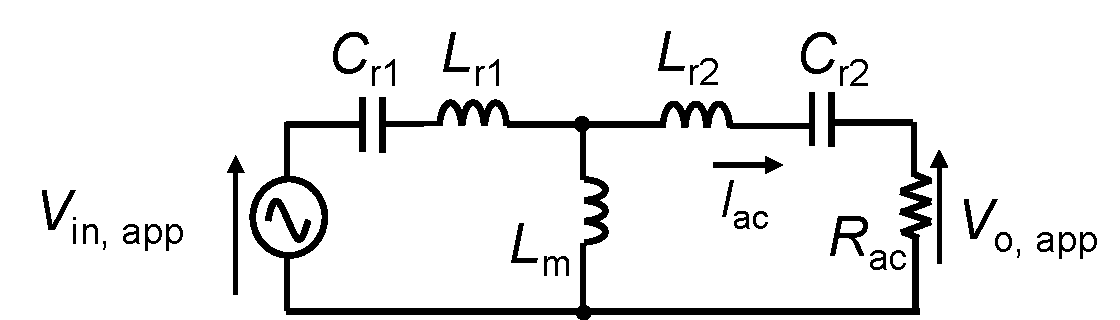
\includegraphics[width=0.7\columnwidth]{figures_chapter2/FHA_Equivalent.pdf} \label{fig:AC_eq}
    }
\caption{First Harmonic Analysis: (a) original circuit, (b) equivalent circuit after FHA.}
\end{figure}

By applying a Fourier series expansion, the fundamental component of the input square-wave voltage $V_{\mathrm{in, app}}(t)$ is extracted as shown in Eq. \ref{eq:fha_vs}:
\begin{equation}
V_{\mathrm{in, app}}(t) = \frac{4}{\pi}V_{\mathrm{in}}\sin(\omega t)
\label{eq:fha_vs}
\end{equation}

The other quantities $V_{\mathrm{out, app}}(t)$, $I_{\mathrm{ac}}(t)$, and $I_{\mathrm{ac}}(rms)$  follow as below, given that $n=1$:
\begin{align}
    V_{\mathrm{out,app}}(t) &= \frac{4V_{\mathrm{in}}}{\pi} \sin(\omega t - \phi) = \frac{4V_{\mathrm{o}}}{\pi}\sin(\omega t - \phi)\\
    I_{\mathrm{ac}}(t) &= \sqrt{2}I_{\mathrm{ac,rms}} \sin(\omega t - \phi) \\
    I_{\mathrm{ac,rms}} &= \frac{\pi}{2\sqrt{2}}I_o
\end{align}

The equivalent AC resistance $R_\mathrm{ac}$ can be expressed by the DC load as follows in Eq. \ref{eq:Rac}:
\begin{equation}
R_{\mathrm{ac}} = \frac{V_{\mathrm{out,app,rms}}}{I_{\mathrm{ac,rms}}} = \frac{8}{\pi^2} \frac{V_O}{I_O} = \frac{8}{\pi^2} R_O \label{eq:Rac}
\end{equation}

The voltage gain $\mathbf{M}_g$ can be obtained from the equivalent circuit in Figure \ref{fig:AC_eq}, denoting $C_{\mathrm{r1}}$ and $L_{\mathrm{r1}}$ as $\mathbf{Z}_1$, $C_{\mathrm{r2}}$ and $L_{\mathrm{r2}}$ as $\mathbf{Z}_2$, and $L_\mathrm{m}$ as $\mathbf{Z}_3$ as shown in Eq. \ref{eq:gain}. It is also important to note that since $n=1$, the resonant tank elements are symmetric for the primary and secondary sides.

\begin{equation}
\mathbf{M}_g(s) = \frac{\mathbf{V_\mathrm{o, app}}(s)}{\mathbf{V_\mathrm{i, app}}(s)} = \frac{\mathbf{V_\mathrm{o}}(s)}{\mathbf{V_\mathrm{in}}(s)} = \frac{(\mathbf{Z}_2 + R_{\mathrm{ac}}) \parallel \mathbf{Z}_3}{\mathbf{Z}_1 + [\mathbf{Z}_3 \parallel (\mathbf{Z}_2 + R_{\mathrm{ac}})]} \cdot \frac{R_{\mathrm{ac}}}{\mathbf{Z}_2 + R_{\mathrm{ac}}}\label{eq:gain}
\end{equation}

The following quantities are introduced as these relate the parameters of the resonant tank, transformer, and the circuit to the voltage gain:
\begin{itemize}
\item The inductance ratio $k$ is defined as the ratio of the magnetizing inductance to the primary resonant inductance, denoted as $k = L_\mathrm{m}/L_\mathrm{r1}$.
\item The quality factor $Q$ is defined as the  characteristic impedance of the resonant tank relative to the load, denoted as $Q = \frac{\sqrt{L_\mathrm{r1}/C_\mathrm{r1}}}{R_\mathrm{ac}}$.
\item The normalized frequency $f_n$ is the ratio between the switching frequency $f_\mathrm{sw}$ and the resonant frequency $f_\mathrm{r}$, denoted as $f_n = \frac{f_\mathrm{sw}}{f_\mathrm{r}}$.
\item The resonance frequency $f_\mathrm{r}$ is the frequency at whcih $M_g = 1$. It can be denoted in terms of the resonant tank as $f_\mathrm{r} = \frac{1}{2\pi \sqrt{L_\mathrm{r1} \cdot C_\mathrm{r1}}}$.
\end{itemize} 

The gain indicated in Eq. \ref{eq:gain} can be then rewritten in terms of the introduced quantities as  shown in Eq. \ref{eq:newgain}:
\begin{equation}
\|M_g(j\omega)\| = \frac{V_\mathrm{o}}{V_\mathrm{in}}=\frac{1}{\sqrt{\left( Q f_{\mathrm{n}} \left( \frac{1}{k} + 2 \right) - \frac{Q}{f_{\mathrm{n}}} \left( \frac{2}{k} + 2 \right) + \frac{Q}{k f_{\mathrm{n}}^3} \right)^2 + \left( \frac{1}{k} - \frac{1}{k f_{\mathrm{n}}^2} + 1 \right)^2}}\label{eq:newgain}
\end{equation}

The gain curve can be shaped by choosing a value for $k$ and $Q$ over $f_n$ which can in turn then give the resonant parameters for the circuit. Shown in Figure \ref{fig:constantQ} is a gain curve shaped by $k$ and in Figure \ref{fig:constantK} is a gain curve shaped by $Q$.

\begin{figure}[h!]
    \centering
    \subfloat[]{
        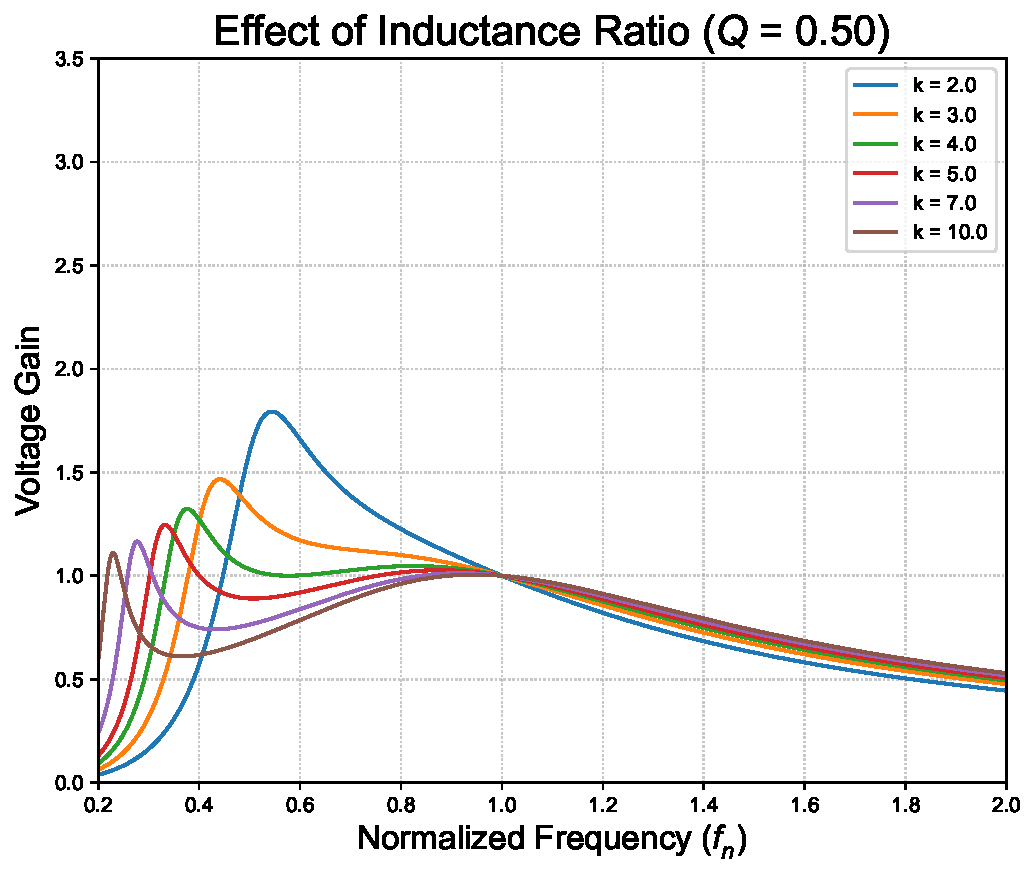
\includegraphics[width=0.5\columnwidth]{figures_chapter2/effect_of_k.pdf} \label{fig:constantQ}
    }
     \subfloat[]{
        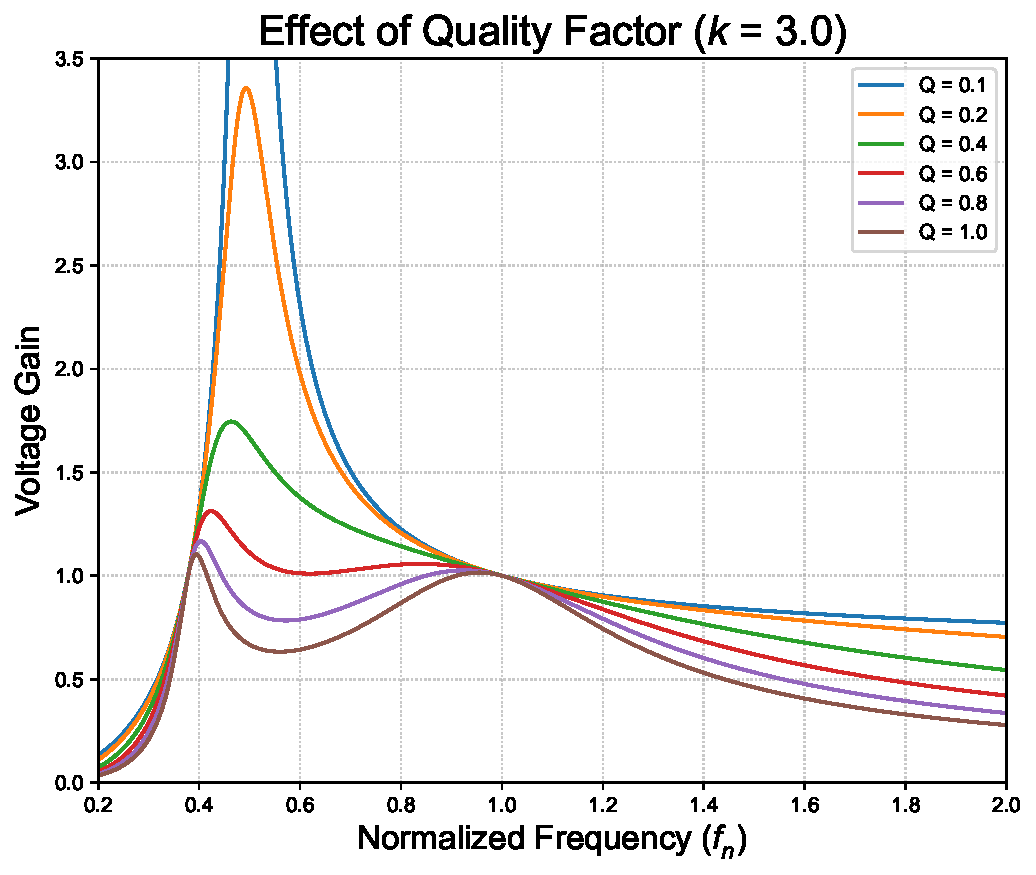
\includegraphics[width=0.5\columnwidth]{figures_chapter2/effect_of_Q.pdf} \label{fig:constantK}
    }
\caption{Gain curves of the CLLC with (a) $Q$ constant, and (b) $k$ constant.}
\end{figure}

A high $k$ value allows the converter to operate over a wider frequency range but inherently necessitates a larger magnetizing inductance, which can increase the peak-to-peak current ripple and bulkiness of the transformer. On the other hand, $Q$ represents the contribution by the load and it can heavily affect the gain curve. Thereore, a carefully selected $Q$ and $k$ is important to ensure a wide operating range for the converter. 

To achieve deadtime, the following constraint is set for the magnetizing inductance \cite{ref19} as shown in Eq. \ref{eq:Lmdt}:
\begin{equation}
L_\mathrm{m} \leq \frac{t_\mathrm{d}}{16C_\mathrm{oss}f_\mathrm{r}}\label{eq:Lmdt}    
\end{equation}

\noindent where $t_\mathrm{d}$ represents the dead time, $C_\mathrm{oss}$ is the output capacitance of one switch, and $f_\mathrm{r}$ is the resonance frequency.

\section{Established Converter Specifications}\label{sec:established}
The final target for this study is a 100 kW, 1000 V to 1000 V converter, operating at a switching frequency of 15 to 30 kHz. With these in mind, an $n$ of 1 is chosen. It is important to note that this study will cover a \textbf{scaled-down} version of this transformer. To ensure that the scalability of this transformer can be assessed in the future, the parameters are scaled down in equal proportions for the voltage and current. This is so that the $R_\mathrm{ac}$ can stay equivalent for both versions and the theoretical voltage gain characteristics derived from the First Harmonic Approximation (FHA) remain perfectly preserved. Because the equivalent DC load resistance ($R_O$) is constant, the quality factor ($Q$) and the inductance ratio ($k$) of the resonant network are unchanged. This guarantees that the scaled-down prototype will exhibit the exact same normalized gain curves and control dynamics as the full-scale system, allowing for an accurate experimental validation of the resonant tank design before addressing the distinct thermal and parasitic challenges of the 100 kW hardware.

Therefore, the $Q$ and $k$ for the application converter are chosen such that the gain curve is as flat as possible around the $f_\mathrm{n} = 1$ across different loads. 

The resonant frequency is set at $30$ kHz, which is the maximum operating frequency for the study. From here, available components at the 1 kW level were used as a baseline first to choose the resonant tank parameters. Given the availability of suitable resonant inductors and capacitors in the local market at this operation, to achieve this resonance frequency, a $C_\mathrm{r1}$ and $L_\mathrm{r1}$ of 1.4 $\upmu$F and 20.1 $\upmu$H is chosen.

The $k$ is chosen as follows. The converter in this study will only be operated at its nominal operating point, at open-loop control, meaning it is desired for the converter to obtain $M_\mathrm{g}=1$ most of the time given a gain curve. From the specifications in Table \ref{tab:converter_specs} the $Q$ at maximum load is $0.467$. 

A gain curve at $Q = 0.467$ is shown in Figure \ref{fig:gainMax}. A $k$ is chosen so that it is flat around the resonant frequency. As long as the desired gain is achievable before the first peak resonance point, then the converter can safely regulate the output voltage within the inductive region. However, in the interest of this study, since only open-loop control will be used to evaluate the prototype at its nominal operating point ($M_\mathrm{g} = 1$), a high inductance ratio of $k = 10$ is selected. Operating strictly near the resonant frequency ($f_\mathrm{n} = 1$) inherently guarantees unity gain regardless of $Q$ and gives maximum flexibility in operating frequency at the maximum power. The gain curve with $k=10$ for all operating $Q$ is shown in Figure \ref{fig:gainAll}. With the whole range, it gives a little margin for fine tuning the operating frequency without deviating the gain from 1.0.

\begin{figure}[h!]
    \centering
    \subfloat[]{
        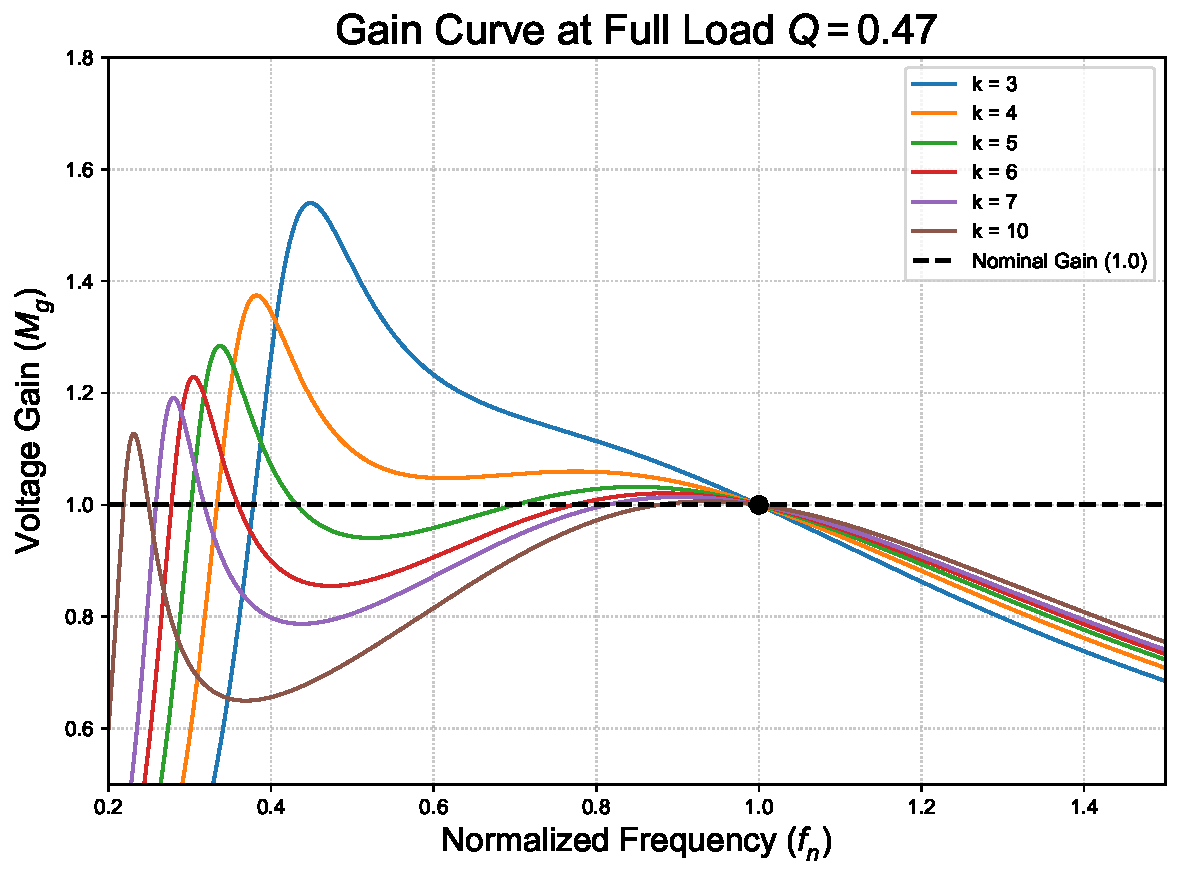
\includegraphics[width=0.5\columnwidth]{figures_chapter2/k_sweep_full_load.pdf} \label{fig:gainMax}
    }
     \subfloat[]{
        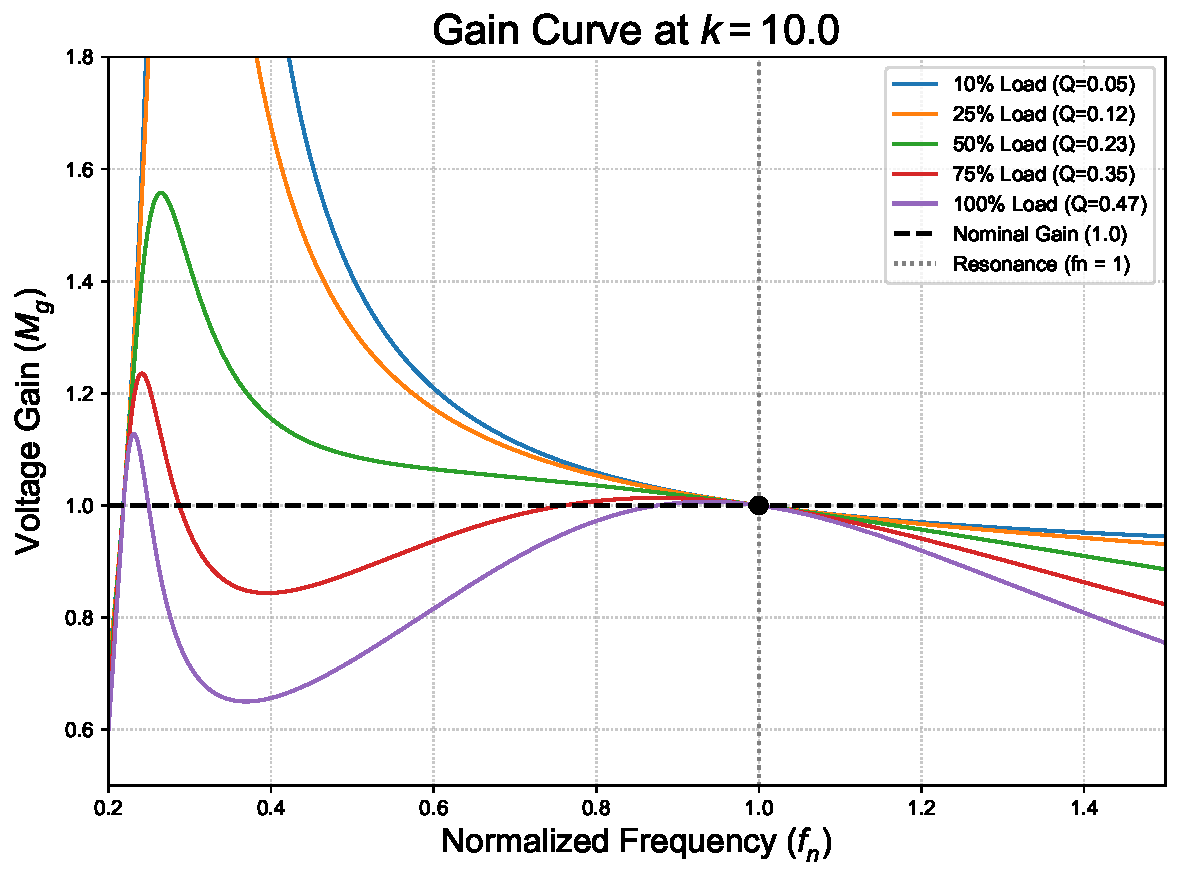
\includegraphics[width=0.5\columnwidth]{figures_chapter2/load_sweep_k10.pdf} \label{fig:gainAll}
    }
\caption{Gain curves of the CLLC at the operating specifications: (a) at max load, or max $Q$, and (b) at $k=10$.}
\end{figure}

\pagebreak
A few simulation waveforms are shown in the Appendix: \nameref{app:simulation}, confirming ZVS operation at 100 kW and 1 kW with the chosen parameters. Moreover, the following specifications are decided for the CLLC Converter, as shown in Table \ref{tab:1kW}.

\begin{table}[h!]
\centering
\caption{Established Converter Specifications for the Small-scale Study}
\label{tab:1kW}
\begin{tabular}{cccc}
\hline
\textbf{Parameter} & \textbf{Symbol} & \textbf{Value} \\
\hline \hline
Input Voltage & $V_{\mathrm{in}}$ & 100 V \\ 
Output Voltage & $V_{\mathrm{out}}$ & 100 V   \\
Switching Frequency & $f_{\mathrm{sw}}$ & 28.5 kHz \\ 
Output Power & $P_\mathrm{O}$ & 1 kW \\
Output Current & $I_\mathrm{O}$ & 10 A \\
\hline
Resonant Frequency & $f_{\mathrm{r}}$ & 30 kHz \\ 
Magnetizing Inductance & $L_\mathrm{m}$ & 200 $\upmu$H   \\
Leakage Inductance & $L_\mathrm{r1}\, L_\mathrm{r2}$ & 20.0 $\upmu$H \\ 
Resonant Capacitance & $C_\mathrm{r1}\, C_\mathrm{r2}$ & 1.4 $\upmu$F \\
Dead Time & $t_\mathrm{d}$ & 200 ns \\
\hline
\end{tabular}
\end{table}





